\section{Communication network}

When a drone is purchased a Slave is setup at the location where the drone is going to operate.
The Slave sends an initializing message to Master, informing Master that a new drone has entered the system.
Master adds the drone with the IP and location of the Slave, along with the drone's unique identifier.
If Master receives an initializing message from a Slave with a drone identifier that is already in the system, it will destroy any session that correlates with that drone. The sessions is destroyed because if one or more sessions are granted and S sends its initializing message it is safe to assume that S either disconnected or crashed and all sessions keys are invalid.
Furthermore if the IP of Slave differs from that of the drone it will be updated.
If a user tries to interact with a drone the system behaves differently. A session key will be made on Slave, this key will be send to Master and giving to the user. With this session key it is possible for the user to communicate directly with the Slave without the Master.

\begin{figure}[!ht]
    \centering 
    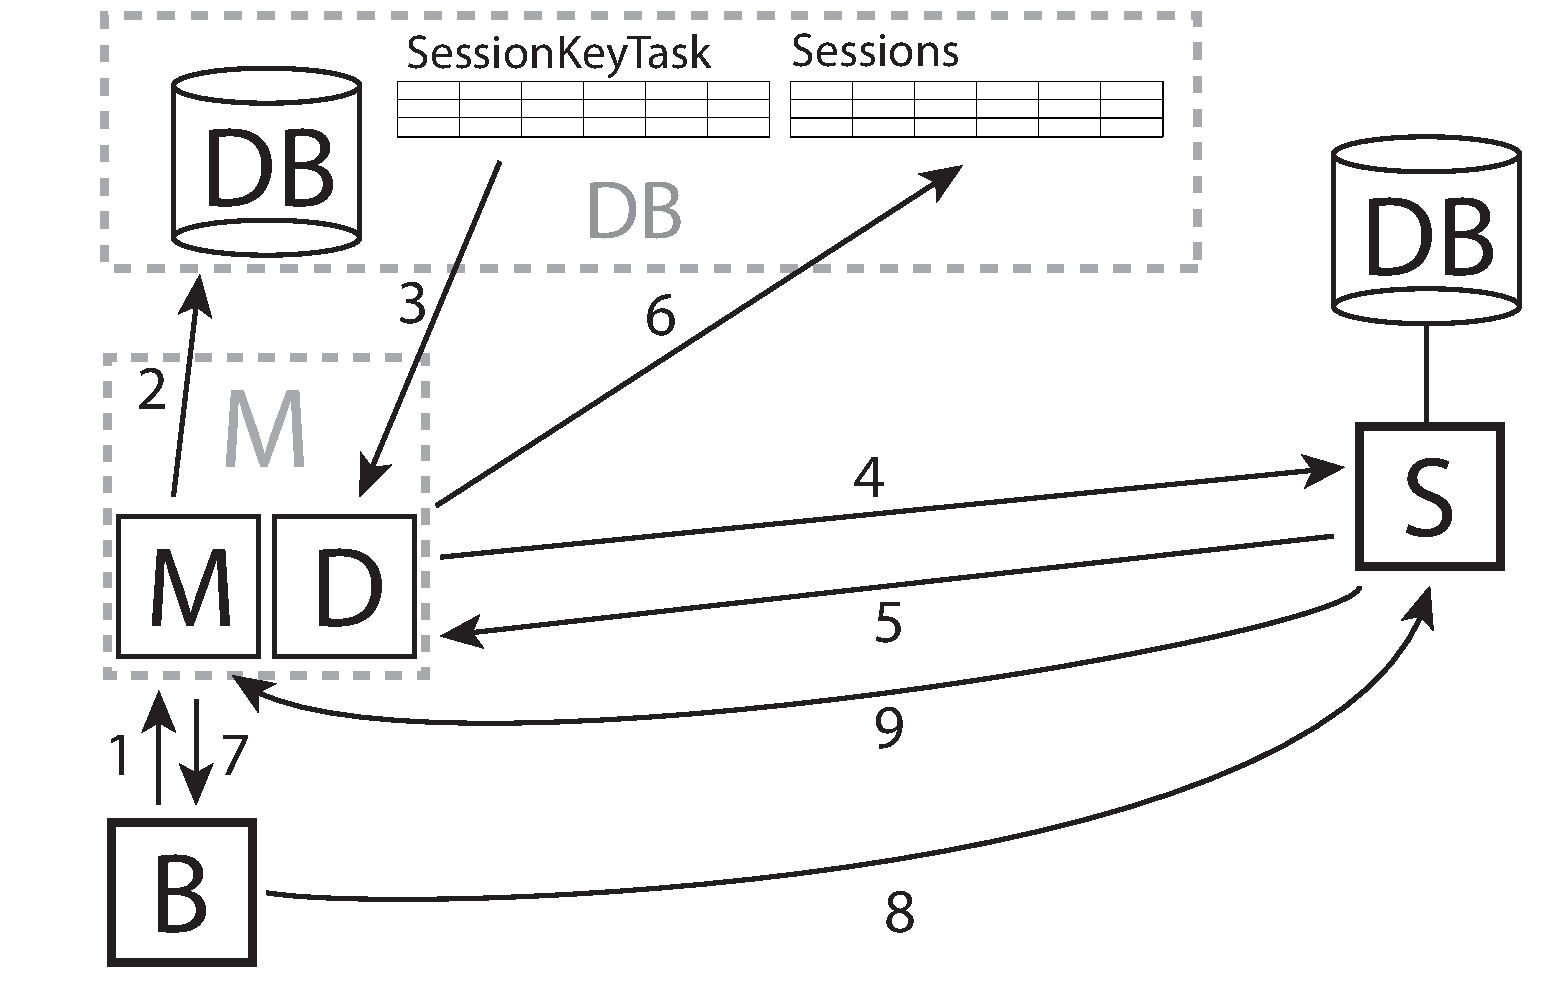
\includegraphics[width=\textwidth]{gfx/sessionkey_communication.pdf}
    \caption{Session key communication between B, M, and S}
    \label{fig:sessionkey_communication}
\end{figure}

This behavior can be seen in figure~\ref{fig:sessionkey_communication}. 


Session keys have been designed for security. If there did not exist session keys in the system it is possible to highjack a drone.

\begin{enumerate}
	\item Request send from B to M about getting a session key to interact with a drone.
	\item M inserts this request in it's database table called SessionKeyTask.
	\item D scans the database table SessionKeyTask, when it sees a new entry it select it and then deletes it from the table.
	\item D requests a session key from S parred with the drone the user wants to interact with.
	\item S makes a random generated string and uses this as the session key. S updates its own database with this session key and then sends it back to D on M.
	\item D inserts the newly received session key into the session table of M.
	\item M then contacts B with the session key.
	\item B uses this session key to access S and through it the drone.
	\item A Timeout happens if B and S does not communicate for 10 seconds.
\end{enumerate}

